\chapter{Polarização da luz}
\textsl{{\sffamily(Versão: \today)}}

\noindent
O termo ``polarização'' refere-se à direção da função de onda, quando a onda é
descrita por funções vetoriais. No caso das ondas eletromagnéticas, esta
direção é a do campo elétrico, e é perpendicular à direção de propagação (como o
é, também, a do campo magnético). Por isso, dizemos que as ondas
eletromagnéticas são transversais. Dentro do plano perpendicular à direção de
propagação em que está confinada, a polarização de uma onda eletromagnética pode
estar orientada em qualquer direção, e pode até variar com o tempo e com a
posição ao longo do caminho da onda.  Chama-se \emph{plano de polarização} de
uma onda eletromagnética ao plano definido pelas direções de polarização e de
propagação (veja a Figura~\ref{fig:polpln}).
\begin{figure}[htb]
    \small
    \sffamily
    {\centering
    \def\zangle{-20}
    \def\xangle{20}

    \begin{tikzpicture}[x=(\xangle:0.75cm), y=(90:1cm), z=(\zangle:1.5cm),
                        >=stealth, line cap=round
                       ]

        \pgfmathsetmacro{\npts}{192}
        \pgfmathsetmacro{\nwvs}{3}
        \pgfmathsetmacro{\dang}{360*\nwvs/\npts}
        \pgfmathsetmacro{\phi}{60}
        \pgfmathsetmacro{\cosphi}{cos \phi}
        \pgfmathsetmacro{\sinphi}{sin \phi}

        \draw [very thin](0,-1,0) -- (0,1,0);
        \draw [very thin](-1,0,0) -- (1,0,0);
        \draw [->] (0,0,0) -- (0,0,\nwvs+0.25) node[below right] {$\vec k$};

        \draw [dashed,fill=gray!25,ultra thin, fill opacity=0.5]
                (\cosphi,\sinphi,0) -- (-\cosphi,-\sinphi,0) --
                (-\cosphi,-\sinphi,\nwvs+.1) -- (\cosphi,\sinphi,\nwvs+.1) --
                cycle;

        \foreach \k [evaluate={%
              \d=int(\k+1/4);
              \i=\k*\dang;
              \j={\i>0 ? \i+\dang : 0};
              \a=\i; 
              \b=\j; 
              \c=int(mod(\k,8)==0 && cos \a != 0); 
              }]
            in {0,...,192}{

            \draw [semithick](\cosphi*cos \a, \sinphi*cos \a, \i/360) -- 
              (\cosphi*cos \b, \sinphi*cos \b, \j/360);

            \ifnum\c=1
                \draw [->] (0,0,\i/360) --
                    ++(\cosphi*cos \a, \sinphi*cos \a, 0);
            \fi
        }
        \node at (\cosphi,\sinphi,0)   [anchor=south] {$\vec E$};
        \node at (\cosphi,\sinphi,0.5) [anchor=south west,yslant=tan(\zangle)] 
          {\footnotesize Plano de polariza\c{c}\~ao};
    \end{tikzpicture}\par
}
\caption{Plano de polarização de uma onda eletromagnética. O campo magnético não
está representado.\label{fig:polpln}}
\end{figure}
Quando a orientação do plano de polarização de uma onda eletromagnética se
mantém constante, dizemos que a onda está polarizada linearmente. Mas também
pode acontecer que o plano de polarização sofra uma rotação em torno da direção
de propagação, completando uma volta completa ao longo de um comprimento de
onda. Nesses casos dizemos que a onda tem polarização circular ou, mais
geralmente, elítica. Vamos já de seguida estudar estas possibilidades.

\section{Polarização linear, polarização circular, polarização elítica}
Numa onda plana com polarização linear, a orientação do plano de polarização
é constante, ou seja, a direção de polarização (que é, recordemos mais uma vez,
a do campo elétrico) deve ser a mesma em todos os pontos do trajeto da onda e em
todos os instantes.

Consideremos uma onda plana sinusoidal com vetor de onda $\vec k$ e frequência
$\omega$. Para simplificar a linguagem, adotamos um referencial com o eixo dos
$z$ orientado segundo o vetor de onda. O plano $xy$ é então perpendicular à
direção de propagação e deve conter o vetor campo elétrico em todos os pontos e
instantes. 


Seja $E_0$ o módulo
da amplitude do campo elétrico desta onda e $\theta$ o ângulo que a direção de
polarização faz com o
eixo dos $x$. Então, o vetor amplitude desta onda é $\vec
E_0=E_0(\cos\theta,\,\sin\theta,\,0)= E_0(\cos\theta\,\he_x+\sin\theta\,\he_y)$,
e a função de onda assume a forma
\begin{equation*}
\vec E(\vec r,t)=E_0(\cos\theta\,\he_x+\sin\theta\,\he_y)
\cos(\vec k\cdot\vec r-\omega t).
\end{equation*}
Podemos ver esta onda como a sobreposição de duas ondas polarizadas linearmente
segundo as direções coordenadas $x$ e $y$ (ver a Figura~\ref{fig:pollin}):
\begin{equation}\label{eq:lpdec}
\vec E(\vec r,t)=\vec E_x(\vec r,t)+\vec E_y(\vec r,t),\qquad\text{com }
\begin{cases}
\vec E_x(\vec r,t)=E_0\cos\theta\,\he_x\,\cos(\vec k\cdot r-\omega t)\\
\vec E_y(\vec r,t)=E_0\sin\theta\,\he_y\,\cos(\vec k\cdot r-\omega t)
\end{cases}
\end{equation}
\begin{figure}[htb]
{\centering
  \def\zangle{320}
  \def\xangle{10}
  \begin{tikzpicture}[x=(\xangle:1cm), y=(90:1cm), z=(\zangle:1.5cm),
                      >=stealth, line cap=round
                     ]

    \pgfmathsetmacro{\npts}{192}
    \pgfmathsetmacro{\nwvs}{2}
    \pgfmathsetmacro{\dang}{360*\nwvs/\npts}
    \pgfmathsetmacro{\phi}{55}
    \pgfmathsetmacro{\cosphi}{cos \phi}
    \pgfmathsetmacro{\sinphi}{sin \phi}

    \draw [very thin,->](0,-1,0) -- (0,1,0) node [right]{$y$};
    \draw [very thin,->](-1,0,0) -- (1,0,0) node [below]{$x$};
    \draw [->] (0,0,0) -- (0,0,\nwvs+0.25) node[below] {$z$};
    \fill [fill=gray!25, fill opacity=0.5]
        (-1.1,-1.05,\nwvs+1) -- (1.,-1.,\nwvs+1) --
        (1.,1.,\nwvs+1) -- (-1.1,1.1,\nwvs+1) -- cycle;
    \draw [ultra thin] (-1,0,\nwvs+1)--(1,0,\nwvs+1);
    \draw [ultra thin] (0,-0.97,\nwvs+1)--(0,0.97,\nwvs+1);
    \draw [<->] (-\cosphi,-\sinphi,\nwvs+1)
    coordinate(e1)--(\cosphi,\sinphi,\nwvs+1)coordinate(e2) node[below right]{$\vec E$};
    \draw [<->,red] (-\cosphi,0,\nwvs+1) coordinate(x1) -- (\cosphi,0,\nwvs+1) coordinate(x2);
    \draw [ultra thin, dashed] (e1)--(x1);
    \draw [ultra thin, dashed] (e2)--(x2) node[yshift=-4mm]{$\vec E_x$};
    \draw [<->,blue] (0,-\sinphi,\nwvs+1)coordinate(y1) -- (0,\sinphi,\nwvs+1)coordinate(y2);
    \draw [ultra thin, dashed] (e1)--(y1);
    \draw [ultra thin, dashed] (e2)--(y2) node[below left]{$\vec E_y$};

    \draw [thin] (0.3,0,\nwvs+1) arc(0:\phi:0.3);
    \path (0.5,0,\nwvs+1) arc(0:\phi/2:0.5) node{$\theta$};
    \draw [thin] (0.8,0,0) arc(0:\phi:0.8);
    \path (0.95,0,0) arc(0:\phi/2:0.95) node{$\theta$};

    \foreach \k [evaluate={%
          \d=int(\k+1/4);
          \i=\k*\dang;
          \j={\i>0 ? \i+\dang : 0};
          \a=\i; 
          \b=\j; 
          \c=int(mod(\k,4)==0 && cos \a != 0); 
          }]
        in {0,...,192}{

        \draw [red](\cosphi*cos \a, 0, \i/360) -- 
          (\cosphi*cos \b, 0, \j/360);

        \draw [blue](0, \sinphi*cos \a, \i/360) -- 
          (0, \sinphi*cos \b, \j/360);

        \draw [very thick](\cosphi*cos \a, \sinphi*cos \a, \i/360) -- 
          (\cosphi*cos \b, \sinphi*cos \b, \j/360);

        \ifnum\c=1
            \draw [ultra thin](0,0,\i/360) --
                ++(\cosphi*cos \a, \sinphi*cos \a, 0);
        \fi
    }

  \end{tikzpicture}\par
}
\caption{Decomposição ortogonal da polarização linear de uma onda. Representa-se
uma onda com polarização linar arbitrária como a soma de duas ondas com
polarizações lineares segundo as direções coordenadas com diferença de fase
nula (linhas finas, representadas a azul e vermelho em impressões a
cores).\label{fig:pollin}}
\end{figure}

A eq.~\eqref{eq:lpdec} mostra que é possível descrever uma onda eletromagnética
plana sinusoidal com polarização linear como a sobreposição de duas ondas com
iguais frequência, vetor de onda e constante de fase, polarizadas linearmente em
duas direções ortogonais do plano perpendicular à direção de propagação.
Estudemos estas sobreposições com mais algum detalhe. Sejam $\vec E_x$ e $\vec
E_y$ duas ondas planas sinusoidais com amplitudes com módulos iguais\footnote{Esta
restrição de igualdade dos módulos das amplitudes permite simplificar a álgebra,
sacrificando-se ligeiramente a generalidade da discussão.}, com igual
vetor de onda (tomado na direção do eixo dos $z$) e igual frequência,
polarizadas linearmente, respetivamente segundo as direções dos eixos dos $x$ e
dos $y$,
\begin{align*}
\vec E_x(\vec r,t)&=\he_x E_0\cos(\vec k\cdot\vec r-\omega t),\\
\vec E_y(\vec r,t)&=\he_y E_0\cos(\vec k\cdot\vec r-\omega t - \delta\varphi).
\end{align*}
Como é a polarização da onda resultante da sobreposição destas duas ondas, em
função da diferença entre as suas fases, $\delta\varphi$?
\begin{description}[leftmargin=0pt,labelindent=0pt]
\item[\textbf{Caso 1, $\bm{\delta \varphi=0}$}]\hfill\\
\begin{minipage}[t]{0.85\linewidth}
Esta é a situação descrita na eq.~\eqref{eq:lpdec}, tomando ondas com amplitudes
com módulos iguais. Neste caso, as duas ondas ortogonais têm em cada ponto e em
cada instante, módulos iguais, e por isso o resultado é uma onda polarizada
linearmente numa direção que faz com o eixo dos $x$ um ângulo de 45$^\circ$, nos
primeiro e terceiro quadrantes.
\end{minipage}\hfill
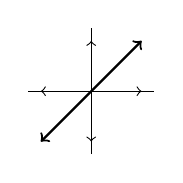
\begin{tikzpicture}[baseline=(current bounding box.north)]
\def\ll{0.8}
\draw (-\ll,0) -- (\ll,0);
\draw (0,-\ll) -- (0,\ll);
\draw [<->] (-0.8*\ll,0)--(0.8*\ll,0);
\draw [<->] (0,-0.8*\ll)--(0,0.8*\ll);
\draw [,thick, <->] (-0.8*\ll,-0.8*\ll) -- (0.8*\ll,0.8*\ll);
\end{tikzpicture}

\item[\textbf{Caso 2, $\bm{\delta\varphi=\pm\pi}$}]\hfill\\
As duas ondas a considerar agora são
\begin{align*}
\vec E_x(\vec r,t)&=\he_x E_0\cos(\vec k\cdot\vec r-\omega t),\\
\vec E_y(\vec r,t)&=\he_y E_0\cos(\vec k\cdot\vec r-\omega t \mp \pi)=
-\he_y E_0\cos(\vec k\cdot\vec r-\omega t),
\end{align*}
\begin{minipage}[t]{0.85\linewidth}
já que adicionar (ou subtrair) $\pi$ ao argumento do cosseno é equivalente a
trocar o sinal ao resultado. As duas ondas têm agora componentes escalares
iguais mas com sinais opostos, de forma que a sua sobreposição é ainda (como no
caso anterior) uma onda polarizada linearmente, numa direção que faz
ainda um ângulo de 45$^\circ$ com o eixo dos $x$, mas agora nos segundo e quarto
quadrantes.
\end{minipage}\hfill
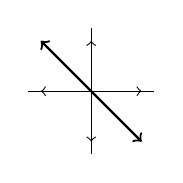
\begin{tikzpicture}[baseline=(current bounding box.north)]
\def\ll{0.8}
\draw (-\ll,0) -- (\ll,0);
\draw (0,-\ll) -- (0,\ll);
\draw [<->] (-0.8*\ll,0)--(0.8*\ll,0);
\draw [<->] (0,-0.8*\ll)--(0,0.8*\ll);
\draw [,thick, <->] (-0.8*\ll,0.8*\ll) -- (0.8*\ll,-0.8*\ll);
\end{tikzpicture}

\item[\textbf{Caso 3, $\bm{\delta\varphi=\pi/2}$}]\hfil\\
A coisa torna-se agora mais interessante. As duas sondas a sobrepor são
\begin{equation}\label{eq:circpol}
\begin{aligned}
\vec E_x(\vec r,t)&=\he_x E_0\cos(\vec k\cdot\vec r-\omega t),\\
\vec E_y(\vec r,t)&=\he_y E_0\cos(\vec k\cdot\vec r-\omega t - \pi/2)=
\he_y E_0\sin(\vec k\cdot\vec r-\omega t),
\end{aligned}
\end{equation}
uma vez que $\cos(x-\pi/2)=\sin x$.
Agora, a razão entre as componentes escalares das duas ondas não é constante, o
que significa que a direção do campo elétrico resultante vai variar de ponto
para ponto e de instante para instante. A onda resultante \emph{não tem}
polarização linear, apesar de ser a sobreposição de duas ondas com polarização
linear. Em cada ponto o vetor campo elétrico vai rodando em torno da direção de
propagação no sentido horário, realizando uma volta completa ao fim de um
período.  A Figura~\ref{fig:circpol} tenta ilustrar o campo elétrico em
diferentes pontos do trajeto da onda, num dado instante.
\begin{figure}[htb]
{\centering
\def\zangle{210}
\def\xangle{-20}
\begin{tikzpicture}[x=(\xangle:1cm), y=(90:1cm), z=(\zangle:1.25cm),
                      				>=stealth, line cap=round,
                              scale=0.8
                     			   ]
\small
\pgfmathsetmacro{\n}{200}
\pgfmathsetmacro{\tm}{850}
\pgfmathsetmacro{\dt}{\tm/\n}
\pgfmathsetmacro{\zm}{4}
\pgfmathsetmacro{\dz}{\zm/\n}

\draw [very thin,->](0,-1,0) -- (0,1,0) node [right]{$y$};
\draw [very thin,->](-1,0,0) -- (1,0,0) node [below]{$x$};
\draw [thick,->] (0,0,0) -- (0,0,1.1*\zm) node[below right] {$z$};

\foreach \k [evaluate={
						\t = \k*\dt;
						\tp = \dt*(\k+1);
						\z=\k*\dz;
						\flag=int(mod(\k,4)==0);
						}] in {0,...,\n}{
		\draw [thin]({cos(\t)},{sin(\t)},\z)--({cos(\tp)},{sin(\tp)},{\z+\dz});
		\ifnum\flag=1
			\draw [thin,->] (0,0,\z) -- ({cos(\t)},{sin(\t)},\z);
		\fi
	}
    \fill [fill=gray!25, fill opacity=0.5]
        (-1.1,-1,\zm+1.5) -- (1.1,-1.1,\zm+1.5) --
        (1.1,1.1,\zm+1.5) -- (-1.1,1,\zm+1.5) -- cycle;
		\draw (0,0,\zm+1.5) circle (1);
		\draw [->] (0,0,\zm+1.5) -- ({cos(\tm)},{sin(\tm)},\zm+1.5)
        node[yshift=-4mm]{$\vec E$};
		\draw [<-] ({1.1*cos(\tm-10)},{1.1*sin(\tm-10},\zm+1.5) 
        arc(\tm-10:\tm+10:1.1);
\end{tikzpicture}\par
}
\caption{Rotação do plano de polarização numa onda com polarização circular
esquerda ($\delta\varphi=\pi/2$).  Note que o módulo do campo elétrico é
uniforme, apenas a sua orientação varia, rodando em torno da direção de
polarização e completando uma volta completa ao longo de um comprimento de onda. 
\label{fig:circpol}}
\end{figure}
(Esta figura foi produzida fixando $t=0$ nas eqs.~\eqref{eq:circpol} e
atribuindo diferentes valores à coordenada $z$ do vetor posição $\vec r$.)
Note-se que, ao contrário do que acontece nas ondas polarizadas linearmente, a
magnitude do campo elétrico permanece constante, apenas a sua orientação varia
de instante para instante e de ponto para ponto. A extremidade da seta que
representa o campo elétrico na onda resultante em cada ponto desenha um círculo,
razão pela qual se chama a este tipo de polarização \emph{polarização circular.}

\item[Caso 4, $\bm{\delta\varphi=-\pi/2}$]\hfill\\
No caso 3, que acabámos de estudar, a fase da componente $x$ estava avançada
relativamente à da componente $y$ em $\pi/2$. Agora temos a situação oposta, é a
componente $y$ que tem a fase avançada. As duas ondas ortogonais são agora
\begin{equation*}
\begin{aligned}
\vec E_x(\vec r,t)&=\he_x E_0\cos(\vec k\cdot\vec r-\omega t)\\
\vec E_y(\vec r,t)&=\he_y E_0\cos(\vec k\cdot\vec r-\omega t + \pi/2)=
-\he_y E_0\sin(\vec k\cdot\vec r-\omega t)
\end{aligned}
\end{equation*}
Os resultados são semelhantes aos obtidos no caso anterior, mas o plano da
polarização da onda resultante roda agora no sentido anti-horário (veja a
Figura~\ref{fig:circpolR})
\begin{figure}[htb]
{\centering
\def\zangle{210}
\def\xangle{-20}
\begin{tikzpicture}[x=(\xangle:1cm), y=(90:1cm), z=(\zangle:1.25cm),
                      				>=stealth, line cap=round,
                              scale=0.8
                     			   ]
\small
\pgfmathsetmacro{\n}{200}
\pgfmathsetmacro{\tm}{850}
\pgfmathsetmacro{\dt}{\tm/\n}
\pgfmathsetmacro{\zm}{4}
\pgfmathsetmacro{\dz}{\zm/\n}

\draw [very thin,->](0,-1,0) -- (0,1,0) node [right]{$y$};
\draw [very thin,->](-1,0,0) -- (1,0,0) node [above]{$x$};
\draw [thick,->] (0,0,0) -- (0,0,1.1*\zm) node[above] {$z$};

\foreach \k [evaluate={
						\t = \k*\dt;
						\tp = \dt*(\k+1);
						\z=\k*\dz;
						\flag=int(mod(\k,4)==0);
						}] in {0,...,\n}{
		\draw [thin]({cos(\t)},-{sin(\t)},\z)--({cos(\tp)},-{sin(\tp)},{\z+\dz});
		\ifnum\flag=1
			\draw [thin,->] (0,0,\z) -- ({cos(\t)},-{sin(\t)},\z);
		\fi
	}
    \fill [fill=gray!25, fill opacity=0.5]
        (-1.1,-1,\zm+1.5) -- (1.1,-1.1,\zm+1.5) --
        (1.1,1.1,\zm+1.5) -- (-1.1,1,\zm+1.5) -- cycle;
		\draw (0,0,\zm+1.5) circle (1);
		\draw [->] (0,0,\zm+1.5) -- ({cos(\tm)},{-sin(\tm)},\zm+1.5)
        node[yshift=2mm]{$\vec E$};
		\draw [->] ({1.1*cos(\tm-10)},{1.1*sin(\tm-10},\zm+1.5) 
        arc(\tm-10:\tm+10:1.1);
\end{tikzpicture}\par
}
\caption{Rotação do plano de polarização numa onda com polarização circular
direita ($\delta\varphi=-\pi/2$).  \label{fig:circpolR}}
\end{figure}
Na situação agora estudada, o sentido da rotação do plano de polarização
relaciona-se com o da propagação da onda pela regra da mão direita. Por isso,
diz-se que neste caso a polarização é \emph{polarização circular direita;} no
caso anterior, em que o plano da polarização roda no sentido horário, falamos de
\emph{polarização circular esquerda.}

\item[Caso genérico, $\bm{\delta\varphi}$ qualquer]\hfill\\
Num caso genérico, com $\delta\varphi$ arbitrário, o resultado da sobreposição
de duas ondas polarizadas linearmente em direções ortogonais é uma onda em que o
campo elétrico roda em torno da direção de propagação como na polarização
linear, mas sobreposta a essa rotação ocorre também uma oscilação (com a
frequência da onda) no módulo do vetor campo elétrico. Assim, a extremidade da
seta que representa em cada ponto o campo desenha uma elipse centrada nesse
ponto. Se as duas ondas a sobrepor têm amplitudes de igual módulo, o eixo maior
da elipse está inclinado 45$^\circ$ relativamente ao eixo dos $x$, nos
quadrantes 1 e 3 ou nos quadrantes 2 e 4 (conforme o valor da diferença de fase
$\delta\varphi$) e esta elipse pode ser percorrida no sentido horário ou
anti-horário, em função também do valor da diferença de fase. Neste caso (ou
quando as as amplitudes das duas componentes da onda resultante não são iguais,
independentemente da diferença de fase), falamos de \emph{polarização elíptica.}
A Figura~\ref{fig:elipol} tenta representar uma onda com polarização elíptica.
\begin{figure}[htb]
{\centering
\def\zangle{210}
\def\xangle{-10}
\begin{tikzpicture}[x=(\xangle:1cm), y=(90:1cm), z=(\zangle:1.25cm),
                      				>=stealth, line cap=round,
                              scale=0.8
                     			   ]
\small
\pgfmathsetmacro{\n}{125}
\pgfmathsetmacro{\tm}{750}
\pgfmathsetmacro{\dt}{\tm/\n}
\pgfmathsetmacro{\zm}{4}
\pgfmathsetmacro{\dz}{\zm/\n}

\draw [very thin,->](0,-1,0) -- (0,1,0) node [right]{$y$};
\draw [very thin,->](-1,0,0) -- (1,0,0) node [above]{$x$};
\draw [thick,->] (0,0,0) -- (0,0,1.1*\zm) node[above] {$z$};

\def\stot{0.707107}
\foreach \k [evaluate={
						\t = \k*\dt;
						\tp = \dt*(\k+1);
						\z=\k*\dz;
						\flag=int(mod(\k,4)==0);
						\x = \stot*(0.6*cos(\t)-sin(\t));
						\y = \stot*(0.6*cos(\t)+sin(\t));
						\xp = \stot*(0.6*cos(\tp)-sin(\tp));
						\yp = \stot*(0.6*cos(\tp)+sin(\tp));
						}] in {0,...,\n}{
		%line
		\draw [thin]({\x},{\y},{\z})--({\xp},{\yp},{\z+\dz});
		%arrows
		\ifnum\flag=1
			\draw [thin,->] (0,0,\z) -- ({\x},{\y},\z);
		\fi
	}
	%Projection plane%%%%%%%%%%%%%%%%%%%%%%%%%
    \fill [fill=gray!25, fill opacity=0.5]
        (-1.,-1,\zm+1.5) -- (1.,-1.1,\zm+1.5) --
        (1.,1.1,\zm+1.5) -- (-1.,1,\zm+1.5) -- cycle;
		%\draw [red] (-1,1,\zm+1.5) -- (1,-1.0,\zm+1.5);
		\begin{scope}[rotate around={45:(0,0,\zm+1.5)}]
		%elipse
		\draw (0,0,\zm+1.5) ellipse (0.6 and 1);
		%Little arrow on the projection plane
		\draw [thin,<-] ({0.6*cos(0)},{sin(0},\zm+1.5) 
        arc(0:25:0.6 and 1);
		\end{scope}
		\draw [thin,->] (-1,0,\zm+1.5) -- ++(2,0,0);
		\draw [thin,->] (0,-1,\zm+1.5) -- ++(0,2,0);
		\draw [thin, dashed] (-1,1,\zm+1.5) -- (1,-1,\zm+1.5);
\end{tikzpicture}\par
}
\caption{Onda com polarização elíptica esquerda. Como na polarização circular, o
campo elétrico roda em torno da direção de propagação ao longo de um período.
Mas, simultaneamente, dá-se uma oscilação do módulo do campo.\label{fig:elipol}}
\end{figure}
\end{description}

Os vários casos estudados estão ilustrados na Figura~\ref{fig:allort}, para os
diferentes valores da diferença de fase $\delta\varphi$.
\begin{figure}[htb]
{\centering
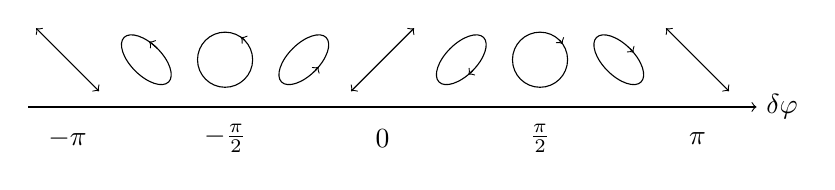
\begin{tikzpicture}
\draw [->](-4.5cm,-0.6) -- (4.75cm,-0.6) node[right] {$\delta\varphi$};
\begin{scope}[xshift=-4cm]
\draw [<->] (-0.4,0.4) -- (0.4,-0.4);
\node at (0,-1) {$-\pi$};
\end{scope}
%
\begin{scope}[xshift=-3cm]
\draw [rotate=-45] (0,0) ellipse(0.4 and 0.2);
\draw [thin,->,rotate=-45] (0,0.2) arc (90:110:0.4 and 0.2);
\end{scope}
%
\begin{scope}[xshift=-2cm]
\draw (0,0) circle (0.35);
\draw [thin,->] (45:0.35) arc (45:55:0.35);
\node at (0,-1) {$-\frac{\pi}{2}$};
\end{scope}
%
\begin{scope}[xshift=-1cm]
\draw [rotate=45] (0,0) ellipse(0.4 and 0.2);
\draw [thin,->,rotate=45] (0,-0.2) arc (270:280:0.4 and 0.2);
\end{scope}
%
\begin{scope}[xshift=0cm]
\draw [<->] (-0.4,-0.4) -- (0.4,0.4);
\node at (0,-1) {$0$};
\end{scope}
%
\begin{scope}[xshift=1cm]
\draw [rotate=45] (0,0) ellipse(0.4 and 0.2);
\draw [thin,->,rotate=45] (0,-0.2) arc (270:260:0.4 and 0.2);
\end{scope}
%
\begin{scope}[xshift=2cm]
\draw (0,0) circle (0.35);
\draw [thin,->] (45:0.35) arc (45:35:0.35);
\node at (0,-1) {$\frac{\pi}{2}$};
\end{scope}
%
\begin{scope}[xshift=3cm]
\draw [rotate=-45] (0,0) ellipse(0.4 and 0.2);
\draw [thin,->,rotate=-45] (0,0.2) arc (90:80:0.4 and 0.2);
\end{scope}
%
\begin{scope}[xshift=4cm]
\draw [<->] (-0.4,0.4) -- (0.4,-0.4);
\node at (0,-1) {$\pi$};
\end{scope}
\end{tikzpicture}\par
}
\caption{Diferentes possibilidades para a polarização da sobreposição de duas
ondas com a mesma amplitude, frequência e comprimento de onda, polarizadas
linearmente em duas direções ortogonais, como função da diferença entre as suas
fases.\label{fig:allort}}
\end{figure}

\section{Luz ``despolarizada'' e luz parcialmente polarizada}
A produção de luz por fontes ``naturais'' (Sol, chamas, lâmpadas de diferentes
tipos, etc) tem sempre uma certa extensão espacial (a luz produzida tem origem
em diferentes pontos do espaço) e temporal (a luz produzida tem origem em
diferentes instantes). Assim, a luz que recebemos de uma dada fonte é a
sobreposição da luz produzida em diferentes pontos da fonte e em diferentes
instantes, em circunstâncias mais ou menos independentes (consoante o tipo
particular de fonte usada). Estas diferentes contribuições para a luz produzida
por uma fonte têm, em geral diferentes características: diferentes comprimentos
de onda (embora as fontes LED e os laser possam ser altamente monocromáticos),
diferentes amplitudes, diferentes fases (também aqui os laser são excepção, uma
vez que os vários processos elementares de emissão ocorrem em fase) e, com
especial relevância para o que agora nos ocupa, diferentes polarizações.
Por esta razão, a polarização da luz natural é quase sempre inobservável; num
raio de luz natural coexistem em sobreposição componentes com diferentes tipos
de polarização e com diferentes orientações, resultando uma média mais ou menos
isotrópica (igual em todas as direções). A direção do campo elétrico num raio de
luz natural (ou seja, a sua polarização) é, assim, inobservável. Chamamos luz
\emph{despolarizada} a uma destas misturas isotrópicas de contribuições de
diferentes polarizações.

Considerando ainda estas sobreposições de luz com diferentes polarizações, pode
também acontecer que a mistura não seja completamente homogénia. As diferentes
componentes com diferentes polarizações podem ter intensidades diferentes,
resultando um feixe que se diz \emph{parcialmente polarizado.} A luz polarizada
e a luz despolarizadas são dois casos particulares extremos (e opostos) de luz
parcialmente polarizada: a primeira, é constituída por uma sobreposição com
100\% de um tipo de polarização e 0\% de todas as outras; a segunda é uma
mistura com iguais frações de \emph{todos} os tipos de polarização.

A luz natural é, em geral, despolarizada. Mas alguns processos óticos operam de
forma diferente consoante o tipo ou a orientação da polarização da luz que neles
participa, podendo, por isso, ficar polarizada. Por exemplo, alguns meios
absorvem mais eficientemente luz com determinadas polarizações; a luz que
atravessa esses meios sofre uma atenuação especial das componentes
correspondentes, ou seja, polariza-se.  Outro exemplo, quando a luz incide numa
superfície que separa dois meios distintos dá-se, como sabemos, a reflexão e a
refração da luz; na reflexão são atenuadas as componentes da luz incidente que
pertencem ao plano de incidência, ficando a luz parcialmente polarizada numa
direção paralela à superfície; na refração ocorre o efeito contrário, e a luz
refratada está parcialmente polarizada numa direção do plano de refração.  Nas
próximas secções estudamos alguns destes processos.

\section{Filtros polarizadores e Lei de Malus}
Um filtro polarizador é qualquer dispositivo ótico que é mais ou menos opaco
conforme o estado de polarização da luz que o atravessa. Os filtros
polarizadores mais simples (aqueles em que nos vamos concentrar nesta secção)
absorvem as componentes da luz incidente com polarização linear numa determinada
direção, mas há também filtros polarizadores para as polarizações circulares.

Um filtro polarizador linear ideal transmite (isto é, \emph{deixa passar})
\emph{toda} a luz incidente com polarização linear numa dada direção (a do
chamado \emph{eixo de transmissão} do filtro) e absorve \emph{toda} a radiação
com polarização linear perpendicular a essa direção\footnote{Na verdade, os filtros
\emph{reais} absorvem alguma da radiação polarizada na direção do eixo de
trasmissão e transmitem alguma da radiação perpendicular a essa direção; mas
vamos supor que estas ineficiências são desprezáveis.}. Muito resumidamente, o
funcionamento destes fitros resulta do facto de serem eletricamente condutores
apenas numa direção; o campo elétrico da luz incidente polarizada nessa direção
acelera os eletrões no filtro, estabelecendo uma corrente elétrica, processo no
qual perde energia, o que se traduz numa diminuição da intensidade da luz;
assim, a luz polarizada na direção em que o filtro é condutor
é absorvida. Em contrapartida, a luz polarizada na direção perpendicular não
gera corrente elétrica (porque nessa direção o filtro é isolador), não fornece
energia ao meio, ou seja, não é absorvida.

Consideremos um feixe de luz polarizada linearmente com intensidade $I_0$ que
incide num filtro polarizador linear. Seja $\theta$ o ângulo entre a direção de
polarização da luz do feixe e a do eixo de transmissão do filtro.
\begin{figure}[htb]
{\centering
\colorlet{crystal}{blue!75}
\def\zangle{-20}
\def\xangle{20}
\begin{tikzpicture}[x=(\xangle:0.75cm), y=(90:1cm), z=(\zangle:1.5cm),
									>=stealth, line cap=round, line join=round,
    								lines/.style={gray!50, thick}, 
    								axis/.style={black, thick},
    								plate/.style={fill, opacity=0.875},
    								markers/.style={orange, thick}]
	\pgfmathsetmacro{\npts}{100}
	\pgfmathsetmacro{\fz}{0}
	\pgfmathsetmacro{\ff}{720}
	\pgfmathsetmacro{\fff}{\ff+720}
	\pgfmathsetmacro{\zf}{2}
	\pgfmathsetmacro{\q}{50}

	\draw [lines] (-1,-1.05,0) -- (-1,1.05,0) -- (1,1,0) -- (1,-1, 0) -- cycle;
	\draw [thin,gray](-1,0,0) -- (1,0,0);
	\draw [thin,gray](0,-1,0) -- (0,1,0);
	\draw (\q:0.6) arc(\q:90:0.6) node [above right,inner sep=2] {$\theta$};
	\draw [-] (0,0,0) -- (0,0,1.*\zf);
	\foreach \k [evaluate={
						 \z = \k * \zf / (\npts);
						 \zn= \z + \zf/(\npts);
						 \f = (\ff - \fz)/(\npts)*\k;
						 \fn = \f +  (\ff - \fz)/(\npts);
						 \x = cos(\q) * cos(\f);
						 \y = sin(\q) * cos(\f);
						 \xn = cos(\q) * cos(\fn);
						 \yn = sin(\q) * cos(\fn);
						 \c=int(mod(\k,5)==0)
						}] in {0,...,\npts} {
		\ifnum\c=1
			\draw [->](0,0,\z) -- (\x,\y,\z);
		\fi
		\draw [thick] (\x,\y,\z) -- (\xn,\yn,\zn);
	}

    \path [crystal!25, plate] 
        (-1,-1.05,\zf) -- (-1,1.05,\zf) -- (1,1,\zf) -- (1,-1, \zf) -- cycle;
    \path [crystal!50, plate] 
        (-1,-1.05,\zf) -- (-1,-1.05,\zf-0.0625) -- (-1,1.05,\zf-0.0625) --
        (-1,1.05, \zf) -- cycle;
    \path [crystal!75, plate] 
        (-1,1.05,\zf) -- (-1,1.05,\zf-0.0625) -- (1,1,\zf-0.0625) -- (1,1, \zf) -- cycle;
    \node [yslant=tan(\xangle), text=crystal!80, below, font=\small] at 
        (-0.4,-1,\zf){Polarizador};
	\draw [blue,thick] (0,-1,\zf)--(0,1,\zf);
	\draw [dashed] ({cos(\q)},{sin(\q)},\zf) -- (0,{sin(\q)},\zf);
	\draw [<->, thin,black!60] ({-cos(\q)},{-sin(\q)},\zf) -- ({cos(\q)},{sin(\q)},\zf);
	\draw [->](0,0,\zf) -- (0,0,2.15*\zf);
	\foreach \k [evaluate={
						 \z =\zf + \zf * \k / \npts;
						 \zn = \z + \zf/\npts;
						 \f = \ff+(\fff-\ff)/\npts * \k;
						 \fn = \f +  (\fff-\ff)/\npts;
						 \y = sin(\q) * cos(\f);
						 \yn = sin(\q) * cos(\fn);
						 \c=int(mod(\k,5)==0)
						}] in {0,...,\npts} {
		\draw [thick] (0,\y,\z) -- (0,\yn,\zn);
		\ifnum\c=1
			\draw [->](0,0,\z) -- (0,\y,\z);
		\fi

	}
\end{tikzpicture}\par
}
\caption{Efeito de um filtro polarizador sobre luz
polarizada.\label{fig:polaroid}}
\end{figure}
Tal como fizemos na secção anterior, podemos escrever a onda incidente como a
sobreposição de duas ondas linearmente polarizadas em direções ortogonais, uma
paralela ao eixo de transmissão do filtro e a outra perpendicular. Temos então
\begin{equation*}
\vec E_0= \he_\parallel E_0\cos\theta+\he_\perp E_0\sin\theta,
\end{equation*}
onde $E_0$ representa o módulo da amplitude da onda incidente, $\hat
e_\parallel$ é um versor paralelo ao eixo de transmissão do filtro
e $\he_\perp$ um versor perpendicular a esse eixo. De acordo com a
definição de filtro polarizador apresentada acima, a primeira destas
componentes vai ser transmitida, e a segunda absorvida. Assim, o campo elétrico
da onda transmitida pelo filtro é dado por
\begin{equation}\label{eq:analized}
\vec E_t=\he_\parallel E_0\cos\theta,
\end{equation}
estando pois polarizado na direção do eixo de transmissão do filtro, e tem
amplitude de módulo $E_t=E_0\cos\theta$. Se elevarmos ao quadrado os
dois lados desta igualdade e os multiplicarmos por $c\varepsilon_0/2$, obtemos
$c\varepsilon_0 E^2_t/2=c\varepsilon_0 E^2_0\cos^2\theta\,/2$. Mas o
termo no primeiro membro é a irradiância da onda transmitida
(eq.~\eqref{eq:irradiance}) e no segundo aparece a da onda incidente. Concluímos
assim que a intensidade da luz trasmitida por um filtro polarizador é uma fração
da da incidente igual ao quadrado do ângulo entre a direção de polarização da
luz incidente e a do eixo de transmissão do filtro,
\begin{equation*}
I_t=I_0\cos^2\theta.
\end{equation*}
Esta constatação tem o nome de \emph{Lei de Malus.}

\subsection{Transmissão de luz não polarizada}
Um feixe luminoso genérico é, em princípio, uma mistura de raios de luz com
diferentes polarizações. Seja $g_0(\theta)d\theta$ a irradiância das
componentes do feixe com polarização segundo direções que fazem com alguma
direção de referência previamente fixada um ângulo compreendido entre $\theta$ e
$\theta+d\theta$. A irradiância total do feixe é a soma destas irradiâncias
parciais, ou seja,
\begin{equation}\label{eq:poldensity}
I_0=\int_0^{\pi} g_0(\theta) d\theta.
\end{equation}
Quando este feixe atravessa um filtro polarizador com o eixo de transmissão
paralelo à direção de referência referida acima, cada uma das suas componentes
será mais ou menos absorvida conforme a orientação da sua polarização. Seja
agora $g_t(\theta)d\theta$ a irradiância da componente do feixe transmitido
com polarização fazendo um ângulo entre $\theta$ e $\theta+d\theta$ com a 
direção do eixo de transmissão do filtro. De acordo com a lei de Malus, temos
\begin{equation*}
g_t(\theta)d\theta=g_0(\theta)d\theta\,cos^2\theta.
\end{equation*}
A intensidade total do feixe transmitido é então
\begin{equation}\label{eq:poltdens}
I_t=\int_0^\pi g_t(\theta)d\theta=\int_0^\pi g_0(\theta)\cos^2\theta d\theta.
\end{equation}
Supondo que o feixe inicial está depolarizado, a função $g_0(\theta)$ é
constante (o feixe incidente tem iguais intensidades de \emph{todas} as
polarizações), $g_0(\theta)=g_0$, e fazendo o integral (neste caso trivial) da
eq.~\eqref{eq:poldensity}, resulta $g_0=I_0/\pi$. Substituindo na
eq.~\eqref{eq:poltdens}, obtemos
\begin{equation*}
I_t=\int_0^\pi g_0\cos^2\theta d\theta=\frac{I_0}{\pi}\int_0^\pi\cos^2\theta
d\theta=\frac12 I_0.
\end{equation*}
Ou seja, quando luz não polarizada incide num filtro polarizador, o feixe
transmitido tem uma irradiância igual a metade da do feixe incidente.


\section{Polarização por reflexão. Ângulo de Brewster}
Como é bem sabido, quando a luz incide na superfície de separação de dois meios
distintos ocorrem os processos da reflexão e da refração. A irradiância do feixe
incidente distribui-se pelos feixes refletido e refratado, de uma forma que
depende do ângulo de incidência, mas que depende também da polarização. Para
simplificar a discussão que se segue, recordemos alguns termos:
\begin{itemize}[itemsep=-1pt,topsep=1pt,parsep=0pt,
                leftmargin=*,
                %itemindent=-1.3em,
                %listparindent=0pt,
]
\item Direções de \emph{incidência,} de \emph{reflexão} e de \emph{refração} são
respetivamente as direções dos raios incidente, refletido e refratado.
\item \emph{Normal} é a direção perpendicular à superfície de separação dos dois
meios no ponto onde se dá a incidência.
\item \emph{Plano de incidência} é o plano que contêm a direção de incidência e
a normal. Este plano contem também as direções de reflexão e de refração e é
perpendicular, no ponto de incidência, à superfície de separação dos dois meios.
\end{itemize}
\begin{figure}[htb]
{\centering
\def\zangle{-20}
\def\xangle{20}
\begin{tikzpicture}[x=(\xangle:0.95), y=(90:1), z=(\zangle:0.95cm)]
\small\sffamily
\clip (-4.1,-1.) rectangle (4.1,1.15);
\coordinate(F1) at (0,0,-9);
\coordinate(F2) at (9,0,0);
\coordinate (O) at (0,0,-0.2);
%\draw [->] (-1,0,0) -- (1,0,0) node[right]{$x$};
%\draw [->] (0,-1,0) -- (0,1,0) node[right]{$y$};
%\draw [->] (0,0,-1) -- (0,0,1) node[right]{$z$};

\def\lx{1.85}
\def\ly{1.75}
\def\lz{2.5}
\def\lyn{-1.0}
\coordinate (zzp) at (0,0,\lz);
\coordinate (zzn) at (0,0,-\lz);
\coordinate (pzz) at (\lx,0,0);
\coordinate (nzz) at (-\lx,0,0);
\coordinate (zpz) at (0,\ly,0);
\coordinate (znz) at (0,\lyn,0);

%incident plane, upper part
\path (F1) -- ($ (F1)!1.5!(zpz) $) coordinate (ypg);
\coordinate (zpn) at (intersection of zzn--(0,2,-\lz) and F1--ypg);
\coordinate (zpp) at (intersection of zzp--(0,2,\lz) and F1--ypg);
%surface, negative x part
\path (F1) -- ($ (F1)!1.5!(nzz) $) coordinate (xng);
\path (F2) -- ($ (F2)!1.5!(zzn) $) coordinate (zng);
\path (F2) -- ($ (F2)!1.5!(zzp) $) coordinate (zpg);
\coordinate (nzn) at (intersection of F1--xng and F2--zng);
\coordinate (nzp) at (intersection of F1--xng and F2--zpg);
%surface, positive x part
\path (F1) -- ($ (F1)!1.5!(pzz) $) coordinate (xpg);
\coordinate (pzn) at (intersection of F1--xpg and F2--zng);
\coordinate (pzp) at (intersection of F1--xpg and F2--zpg);
%incident plane, lower part
\path (F1) -- ($ (F1)!1.5!(znz) $) coordinate (yng);
\coordinate (znn) at (intersection of zzn--(0,-2,-\lz) and F1--yng); 
\coordinate (znp) at (intersection of zzp--(0,-2,\lz) and F1--yng);
%
\path (zpn) --++(0,0.0,-0.1) node [anchor=south west, yslant=-0.12] {Plano de incid\^encia};
%incidence plane, negative z
\fill [gray!20, fill opacity=0.7] (zzn) -- (znn) -- (znp) -- (zzp) -- cycle;
%surface, positive x
\fill [gray!70, fill opacity=0.7] (zzn) -- (pzn) -- (pzp) -- (zzp) -- cycle;
\draw [thin] (zzn) -- (pzn) -- (pzp) -- (zzp);
\draw (O) -- ($ (znz)!0.3!(znp) $) coordinate(p);
\draw [thin,->] (O) -- ($ (O)!0.4!(p) $);
%incidence plane, positive z
\fill [gray!20, fill opacity=0.7] (zzn) -- (zpn) -- (zpp) -- (zzp) -- cycle;
%normal
\draw [dashed] (0,\lyn,-0.2) -- (0,\ly,-0.2);
%surface, negative x
\fill [gray!70, fill opacity=0.7] (zzn) -- (nzn) -- (nzp) -- (zzp) -- cycle;
\draw [thin] (zzn) -- (nzn) -- (nzp) -- (zzp);
\coordinate (a) at ($ (zpn)!0.4!(O) $);
\draw [->] (a) -- ($ (a)!0.4cm!(F2) $); 
\coordinate (b) at ($ (O)!0.6!(zpp) $);
\draw [->] (b) -- ($ (b)!0.4cm!(F2) $);
%Incident polarization
\draw [->] (a) -- ($ (a)!-0.4cm!(F2) $) node [left,inner sep=1] {\scriptsize$\epsilon_n$};
\draw [->] (a) -- +(40:0.35) node [above,inner sep=1] {\scriptsize$\epsilon_p$};
\draw [->] (a) -- +(220:0.35);
%reflected polarization
\draw [->] (b) -- ($ (b)!-0.4cm!(F2) $) node [above, inner sep=3]
    {\scriptsize$\epsilon_n$};
\draw [->] (b) --+(115:0.3) node[above left,inner sep=1]{\scriptsize$\epsilon_p$};
\draw [->] (b) --+(295:0.3);
%incident and reflected rays
\draw (zpn) -- (O) -- (zpp);
\draw [thin,->] (zpn) -- ($ (zpn)!0.75!(O) $);
\draw [thin,->] (O) -- ($ (O)!0.3!(zpp) $);
\path (nzn) -- (nzp) node [midway, below, sloped, yslant=-0.025] {Superf\'icie refletora};
\end{tikzpicture}\par
}
\caption{Refração e reflexão da luz numa interface entre meios distintos. Estão
representadas a direção normal (a tracejado) os raios incidente, refratado e
refletido e duas componentes da polarição de dois dos raios, na direção
perpendicular ao plano de incidência ($\epsilon_n$) e na perpendicular à
propagação dentro desse plano ($\epsilon_p$).\label{fig:rfl_rfr}}
\end{figure}
Os três raios envolvidos neste processo (incidente, refletido e refratado) estão
todos no plano de incidência. As suas polarizações (quer os raios estejam
polarizados, parcialmente polarizados ou não polarizados) são perpendiculares ao
próprio raio. Para as escrever, podemos decompô-las numa direção perpendicular
ao plano de incidência (componente~$n$) e noutra que, pertencendo ao plano de
incidência, é ainda assim perpendicular ao raio em causa (componente~$p$). As
componentes da polarizção nestas duas direções estão representadas na
Figura~\ref{fig:rfl_rfr} (identificadas com os símbolos $\epsilon_n$ e
$\epsilon_p$) para os raios incidente e refletido.

Por razões que se prendem com detalhes da interação entre a matéria e a radiação
(e que não serão aqui discutidas), as componentes~$p$ da polarização do raio
incidente são perferencialmente transmitidas ao raio refratado. O raio refletido
tem, por isso, essas componentes especialmente atenuadas. Se a luz incidente é
luz despolarizada, então o raio refletido estará parcialmente polarizado
na direção~$n$, a direção perpendicular ao plano de incidência. Assim, os
reflexos da luz natural na superfície dos lagos ou do mar, as nossas imagens
refletidas nos espelhos, o brilho das bolas de bilhar, etc, são todos
constituidos por luz parcialmente polarizada.

A intensidade deste efeito de encaminhamento das componentes~$p$ da polarização
da luz incidente para o raio refratado, reduzindo por essa via a sua presença no
raio refletido, depende do ângulo de incidência. Para uma dada interface entre
dois meios, há uma direção de incidência da luz para a qual as componentes~$p$
da polarização da radiação incidente são \emph{totalmente} transmitidas ao raio
refratado. Quando isto acontece, o raio refletido fica, naturalmente, totalmente
polarizado, com polarização linear na direção~$n$. O ângulo de incidência para o
qual esta situação ocorre chama-se \emph{ângulo de Brewster}. 

Por razões que se prendem também com o mecanismo que causa este processo
de distribuição diferenciada das polarizações~$p$ e~$n$ pelos raios refletido e
refratado, acontece que quando a incidência se faz segundo o ângulo de Brester
(e, portanto, quando o raio refletido resulta totalmente polarizado), as
direções de refração e reflexão são perpendiculares. Este facto permite deduzir
facilmente uma expressão para o valor do ângulo de Brewster para uma dada
interface, que vamos fazer já a seguir.

\noindent
\begin{minipage}[t]{0.75\linewidth}
Consideremos dois meios contíguos com
índices de refração~$n_1$ e~$n_2$, e um raio de luz que propagando-se no
primeiro, incide num dado ponto da superfície de contacto que os separa, segundo
uma direção que faz com a normal no ponto de incidência um ângulo igual ao
ângulo de Brewster (veja a figura ao lado).
De acordo com a lei de Snell, a relação entre o ângulo de incidência
($\theta_B$) e de refração ($\theta_r$) é
\begin{equation*}
n_1\sin\theta_B=n_2\sin\theta_r.
\end{equation*}
\end{minipage}\hfill
\begin{tikzpicture}[baseline=(current bounding box.north)]
\small
\draw [thick] (1.5,0)--(-1.5,0) node [anchor=south west]{$n_1$} node[anchor=north west]{$n_2$};
\draw [dashed] (0,-1.4)--+(0,2.5);
\draw [->-] (150:1.5) -- (0,0); \draw [->-] (0,0) -- (30:1.5);
\draw [thin](0,0.6) arc (90:150:0.6) node [shift={(0.5mm,4mm)}]{$\theta_B$};
\draw [thin](0,0.5) arc (90:30:0.5) node [shift={(-0.3mm,3.5mm)}] {$\theta_B$};
\draw [->-] (0,0)--(300:1.5);
\draw [thin] (0,-0.5) arc(270:300:0.5) node [shift={(-0mm,-3mm)}] {$\theta_r$};
\coordinate (q) at (345:1.4142*0.3);
\draw [thin] (300:0.3) -- (q) --(30:0.3);
\end{tikzpicture}\\[3mm]
Mas, como as direções de reflexão e de refração são perpendiculares (e como,
pela lei da reflexão, o ângulo de reflexão é tabém igual a $\theta_B$), 
\begin{equation*}
\theta_B+90^\circ+\theta_r=180^\circ\implies
\theta_r=90^\circ-\theta_B\implies
\sin\theta_r=\sin(90\circ-\theta_B)=\cos\theta_B.
\end{equation*}
Substituindo acima, obtemos
\begin{equation*}
n_1\sin\theta_B=n_2\cos\theta_B,
\end{equation*}
ou seja,
\begin{equation*}
\tan\theta_B=\frac{n_2}{n_1}.
\end{equation*}




\section{Aplicações na optometria e para as imagens~3D}
Porque na reflexão especular ocorre polarização (parcial ou total) da luz, o
brilho da luz do sol refletida nas superfícies dos lagos ou do mar ou nas
carroçarias dos carros é constituído por luz polarizada. Como as superfícies
que produzem estes reflexos tendem a estar mais ou menos horizontais, a luz
refletida tem polarização mais ou menos horizontal também e pode ser fortemente
atenuada usando filtros polarizadores com o eixo de transmissão orientado
verticalmente. Esta possibilidade é aproveitada por diversos modelos de óculos
de sol comerciais. É igualmente usada em alguns modelos de oftalmoscópio e
outros instrumentos para exame visual do interior do globo ocular, para
atenuar os reflexos muito intensos da córnea.

A técnologia atualmente mais difundida para a visualização de filmes 3D usa
também luz polarizada. No ecrã da sala de cinema, são projetados
simultaneamente \emph{dois} filmes ligeiramente diferentes, que mostram a ação
tal como ela seria percebida por cada olho de uma pessoa que a testemunhasse, e
cada um destes filmes é projetado com luz polarizada: para um usa-se luz
polarizada circularmente no sentido dextro, para o outro luz polarizada
circfularmente no sentido esquerdo. Por outro lado, as lentes dos óculos que se
usam para ver esses filmes têm lentes polarizadoras circulares com orientações
simétricas também.  Deste modo, cada olho do espetador só vê um dos filmes a ser
projetado, cada olho só vê o que veria se o espetador estivesse efetivamente
presente na cena. A partir daqui, entra em ação a parte neurológica do sistema
visual, e o cérebro constrói a partir das imagens (ligeiramente
diferentes) captadas pelos dois olhos a sensação de profundidade.

\newpage
\section*{Ondas eletromagnéticas --- Resumo}
\tobedone{}
%\section{Apêndice: figuras de Lissajous com frequência única}
%\label{sec:lissajous}
%Consideremos o movimento de um ponto material no plano $xy$ cujas coordenadas
%são dadas por 
%\begin{align}\label{eq:mcu}
%x(t)&=r\cos\omega t&y(t)=r\sin\omega t,
%\end{align}
%com $r$ e $\omega$ constantes positivas. É claro que este ponto descreve um
%movimento circular uniforme, com raio $r$ e velocidade angular $\omega$ (veja a
%Figura~\ref{fig:mcu}).
%\begin{figure}[htb]
%{\centering
%\begin{tikzpicture}
%  \small
%  \coordinate (O) at (0,0);
%  \draw [->] (-1.5,0) -- (1.5,0);
%  \draw [->] (0,-1.5) -- (0,1.5);
%  \def\r{1.2}
%  \def\theta{50}
%  \draw [thin] (O) circle (\r);
%  \fill (\theta:\r) coordinate(P) circle(0.1);
%  \draw [thin,->] (0:\r+.185) arc (0:\theta:\r+.185);
%  \node at (0.5*\theta:\r+0.2) [anchor=west] {$\omega t$};
%  \draw [thin, densely dashed] (O-|P)node[below]{$x$} -- (P) --
%        (P-|O) node [left]{$y$};
%  \draw [thin] (O) -- (P) node [midway, shift={(-.1,.1)}] {$r$};
%\end{tikzpicture}\par
%}
%\caption{Movimento circular e uniforme de um ponto com coordenadas que dependem
%do tempo de acordo com as eqs.~\eqref{eq:mcu}.\label{fig:mcu}}
%\end{figure}
%Tendo em conta que $\sin\theta=\cos(\theta-\pi/2)$, as expressões das
%coordenadas do ponto em estudo, das eqs.~\eqref{eq:mcu}, podem também
%escrever-se como
%\begin{align}
%x(t)&=r\cos\omega t& y(t)&=r\cos(\omega t-\pi/2).
%\end{align}
%
%Façamos agora uma generalização destas expressões, substituindo o valor $\pi/2$
%na segunda igualdade por um parâmetro genérico $\varphi,$ e analisemos as
%trajetórias da família definida pelas igualdades
%\begin{align}\label{eq:mcu2}
%x(t)&=r\cos\omega t& y(t)&=r\cos(\omega t-\varphi).
%\end{align}
%O caso $\varphi=\pi/2$ é o que já vimos. A trajetória correspondente é uma
%circunferência descrita no sentido anti horário. Mas há outras possibilidades.
%Por exemplo, com $\varphi=0$ tem-se $x(t)=y(t);$ a trajetória resultante é então
%um segmento de reta com inclinação 45$^\circ$, percorrido pelo ponto material
%alternadamente num sentido e no sentido inverso.  Com $\varphi=\pi$, a situação
%é muito semelhante (mas agora $y(t)=-x(t)$); resulta uma trajetória também
%retilínea, mas com inclinação $-45^\circ$. Para $\varphi=-\pi/2$ resulta
%novamente uma trajetória circular, mas descrita em sentido horário. Mais em
%geral, a trajetória resultante é uma elipse mais ou menos excêntrica, com uma
%inclinação $\pm45^\circ$\footnote{O applet geogebra \texttt{lissajous} em
%\texttt{https://ggbm.at/zbC56YsK} ajuda na exploração
%das várias possibilidades.}.  A Figura~\ref{fig:lsjx_examples} ilustra os casos
%agora referidos e ainda o caso $\varphi=\pi/4$.
%\begin{figure}[htb]
%{\centering
%\begin{tikzpicture}
%    \small
%	\def\r{0.8}
%	\def\q{40}
%	\begin{scope}[xshift=-5cm]
%		\draw [->,thin] (-1,0) -- (1,0);
%		\draw [->,thin] (0,-1) -- (0,1);
%		\draw [thin] (0,0) circle(0.8);
%		\fill(\q:\r) circle(0.05);
%		\draw [->] (\q-10:\r+0.2) arc(\q-10:\q+10:\r+.2);
%		\node at (0,-1.2) {$\varphi=\pi/2$};
%	\end{scope}
%	\begin{scope}[xshift=-2.5cm]
%		\draw [->,thin] (-1,0) -- (1,0);
%		\draw [->,thin] (0,-1) -- (0,1);
%		\draw [thin] (0,0) circle(0.8);
%		\fill(\q:\r) circle(0.05);
%		\draw [->] (\q+10:\r+0.2) arc(\q+10:\q-10:\r+.2);
%		\node at (0,-1.2) {$\varphi=-\pi/2$};
%	\end{scope}
%	\begin{scope}[xshift=0cm]
%		\draw [->,thin] (-1,0) -- (1,0);
%		\draw [->,thin] (0,-1) -- (0,1);
%		\draw (225:\r) -- (45:\r);
%		\fill (45:0.5)coordinate(p) circle(0.05);
%		\path (p)--++(225:0.2)--++(135:0.15) coordinate(q);
%		\draw [<->] (q) --++(45:0.4);
%		\node at (0,-1.2) {$\varphi=0$};
%	\end{scope}
%	\begin{scope}[xshift=2.5cm]
%		\draw [->,thin] (-1,0) -- (1,0);
%		\draw [->,thin] (0,-1) -- (0,1);
%		\draw (135:\r) -- (315:\r);
%		\fill (135:0.5)coordinate(p) circle(0.05);
%		\path (p)--++(315:0.2)--++(45:0.15) coordinate(q);
%		\draw [<->] (q) --++(135:0.4);
%		\node at (0,-1.2) {$\varphi=\pi$};
%	\end{scope}
%	\begin{scope}[xshift=5cm]
%		\draw [->,thin] (-1,0) -- (1,0);
%		\draw [->,thin] (0,-1) -- (0,1);
%    \draw [domain=0:360,samples=50,variable=\t] 
%      plot ({\r*cos(\t)},{\r*cos(\t-30)});
%    \fill ({\r*cos(72)},{\r*cos(42)}) circle(0.05);
%
%    \draw [->,domain=72:88,samples=5,variable=\t] 
%        plot ({(\r+.2)*cos(\t)},{(\r+.2)*cos(\t-30)});
%		\node at (0,-1.2) {$\varphi=\pi/6$};
%    \draw [thin,dashed]
%    ({\r*cos(195)},{\r*cos(165)})--({\r*cos(15)},{\r*cos(-15)});
%    \draw (0:0.6) arc(0:45:0.6) node [shift=({1mm,0.75mm}),anchor=north west]
%            {$45^\circ$};
%	\end{scope}
%\end{tikzpicture}\par
%}
%\caption{Alguns exemplos de sobreposição ortogonal de dois movimentos
%oscilatórios com a mesma frequência e amplitude.\label{fig:lsjx_examples}}
%\end{figure}
%
%As figuras planas resultantes de sobreposição de movimentos oscilatórios em
%direções perpendiculares chama-se \emph{Figuras de Lissajous.} Nestes
%apontamentos consideramos apenas o caso em que as frequências de ambos os
%movimentos são iguais, por ser o relevante para o estudo da polarização elítica.
%
%Estudámos aqui a situação mais simples, em que as amplitudes dos dois movimentos
%oscilatórios são iguais. Mas, no essencial, as coisas não se alteram grandemente
%quando as amplitudes são diferentes, excepto no seguinte:
%\begin{enumerate}
%\item
%  Se as amplitudes dos dois movimentos são diferrentes, a trajetória resultante
%  nunca chega a ser exatamente circular, permanece sempre elítica acom maior ou
%  menor excentricidade;
%\item
%  Se as amplitudes dos dois movimentos são diferentes, a inclinação do eixo da
%  elipse pode tomar outros valores para além de $\pm45^\circ$, obtidos acima.
%\end{enumerate}
